% lecture19.tex — Euler Characteristics, Triangulations, and Cobordisms

\section{Euler Characteristics and Triangulations}

\begin{definition}{Triangulation}{triangulation}
    A \emph{triangulation} of a manifold is a subdivision into \emph{simplices}, the higher-dimensional generalization of triangles.
\end{definition}

\begin{example}{Triangulation of $T^2$}{torus-triangulation}
    The torus $T^2$, viewed as a square with opposite sides identified, can be triangulated by adding a diagonal, yielding $1$ vertex, $3$ edges, and $2$ triangular faces.
\end{example}

\begin{center}
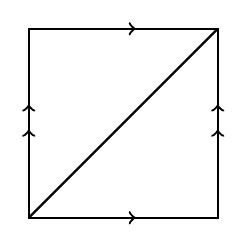
\begin{tikzpicture}[scale=1.6]
    % Square boundary
    \draw[thick] (0,0) -- (1.5,0) -- (1.5,1.5) -- (0,1.5) -- cycle;
    % Diagonal
    \draw[thick] (0,0) -- (1.5,1.5);
    % Single arrow on top/bottom edges
    \draw[thick,->] (0.7,0) -- (0.85,0);
    \draw[thick,->] (0.7,1.5) -- (0.85,1.5);
    % Double arrow on left/right edges (two stacked arrowheads)
    \draw[thick,->] (0,0.55) -- (0,0.7);
    \draw[thick,->] (0,0.75) -- (0,0.9);
    \draw[thick,->] (1.5,0.55) -- (1.5,0.7);
    \draw[thick,->] (1.5,0.75) -- (1.5,0.9);
\end{tikzpicture}
\end{center}

\begin{theorem}{Euler Characteristic via Triangulation}{euler-triangulation}
    If $M$ is an $m$-dimensional triangulated manifold, then
    \[
        \chi(M) = \sum_{j=0}^{m} (-1)^j \cdot \#(j\text{-dimensional faces}).
    \]
\end{theorem}

\begin{proof}
    Given a triangulation, we can construct a vector field $v$ on $M$ with exactly one zero on each face, where the zero on a $j$-dimensional face has index $(-1)^j$:
    \begin{center}
    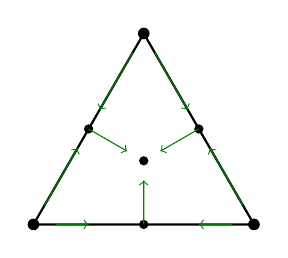
\begin{tikzpicture}[scale=1.4]
        \coordinate (A) at (0,0);
        \coordinate (B) at (2,0);
        \coordinate (C) at (1,1.732);
        \coordinate (mAB) at (1,0);
        \coordinate (mBC) at (1.5,0.866);
        \coordinate (mCA) at (0.5,0.866);
        \coordinate (F) at (1,0.577);
        \draw[thick] (A) -- (B) -- (C) -- cycle;
        % Zeros
        \fill (A) circle (1.5pt);
        \fill (B) circle (1.5pt);
        \fill (C) circle (1.5pt);
        \fill (mAB) circle (1.2pt);
        \fill (mBC) circle (1.2pt);
        \fill (mCA) circle (1.2pt);
        \fill (F) circle (1.2pt);
        % Flow along edges: vertex (source) -> edge midpoint (saddle, stable)
        \draw[->,green!50!black] (0.2,0) -- (0.5,0);
        \draw[->,green!50!black] (1.8,0) -- (1.5,0);
        \draw[->,green!50!black] (0.1,0.173) -- (0.4,0.693);
        \draw[->,green!50!black] (0.9,1.559) -- (0.6,1.039);
        \draw[->,green!50!black] (1.9,0.173) -- (1.6,0.693);
        \draw[->,green!50!black] (1.1,1.559) -- (1.4,1.039);
        % Flow into face center from edge midpoints (saddle, unstable -> sink)
        \draw[->,green!50!black] (mAB) -- (1,0.4);
        \draw[->,green!50!black] (mBC) -- (1.15,0.664);
        \draw[->,green!50!black] (mCA) -- (0.85,0.664);
    \end{tikzpicture}
    \end{center}
    The theorem then follows from Poincar\'e--Hopf.
\end{proof}

\section{Cobordisms (extra topic)}

Much of our discussion so far can be generalized to intersection theory even when the dimensions are not complementary.

Suppose $M_1, M_2 \subset N$ are compact manifolds (of not necessarily complementary dimension). Then, after some homotopy to make the intersection transverse, $M_1 \cap M_2$ is a manifold of dimension $m_1 + m_2 - n$.

Under a homotopy of $M_1$ (or $M_2$), $M_1 \cap M_2$ may change shape, but it remains in the same \emph{cobordism class}: tracking the intersection across the homotopy traces out a manifold inside $N \times I$ whose boundary is the two intersections at times $0$ and $1$.

\begin{definition}{Cobordant Manifolds}{cobordant}
    Two manifolds $M, M'$ of the same dimension are \emph{cobordant} if there is a compact manifold $W$ with boundary $\partial W \cong M \sqcup M'$.
\end{definition}

Being cobordant is an equivalence relation, and we call the equivalence classes \emph{cobordism classes}. They form an abelian group under disjoint union.

\begin{definition}{Cobordism Groups}{cobordism-groups}
    Let $\Omega_n^O$ be the \emph{unoriented cobordism group} of $n$-manifolds, and let $\Omega_n^{SO}$ be the \emph{oriented cobordism group} of oriented $n$-manifolds (and oriented cobordisms).
\end{definition}

The Cartesian product defines a multiplication, so
\[
    \Omega_*^O := \bigoplus_{n \geq 0} \Omega_n^O \quad \text{and} \quad \Omega_*^{SO} := \bigoplus_{n \geq 0} \Omega_n^{SO}
\]
are graded algebras.

\begin{example}{Zero-Dimensional Cobordism Groups}{cobordism-zero-dim}
    \[
        \Omega_0^O \cong \Z/2 \quad (\text{generated by a point}), \qquad \Omega_0^{SO} \cong \Z \quad (\text{generated by a signed point}).
    \]
\end{example}

These are exactly where our mod 2 and oriented intersection theory took values!

\subsection{Thom's Theorem}

This is out of the scope for this course, but Ren\'e Thom proved in 1954:

\begin{theorem}{Thom's Theorem (Unoriented Cobordism)}{thom}
    \[
        \Omega_*^O \cong \mathbb{F}_2[x_i \mid i \geq 1,\ i \neq 2^j - 1],
    \]
    a polynomial algebra with one generator $x_i$ in each dimension $i \neq 2^j - 1$. For even $i$, we may take $x_i = [\R P^i]$.
\end{theorem}

Explicitly, in low dimensions:
\[
    \Omega_0^O \cong \Z/2, \quad \Omega_1^O \cong 0, \quad \Omega_2^O \cong \Z/2, \quad \Omega_3^O \cong 0, \quad \Omega_4^O \cong \Z/2 \oplus \Z/2, \quad \Omega_5^O \cong \Z/2, \ldots
\]

For oriented cobordisms, it is known that, modulo torsion,
\[
    \Omega_*^{SO} \otimes \Q \cong \Q[y_{4i} \mid i \geq 1], \quad \text{where } y_{4i} = [\mathbb{C} P^{2i}],
\]
and
\[
    \Omega_0^{SO} \cong \Z, \quad \Omega_1^{SO} \cong 0, \quad \Omega_2^{SO} \cong 0, \quad \Omega_3^{SO} \cong 0, \quad \Omega_4^{SO} \cong \Z, \quad \Omega_5^{SO} \cong \Z/2, \ldots
\]
